%*****************************************
\chapter{Einführung in die Soziale Netzwerke}\label{ch:SNA}
%*****************************************
Um zu verstehen, warum Soziale Netzwerke analysiert werden, sollte zunächst die Frage geklärt werden, was ein Soziales Netzwerk ist. Hierfür existieren zwei Definitionen, eine gehört dem Bereich der Soziologie an und die andere dem Bereich des Internets. \\
In der Soziologie definiert, ist ein soziales Netzwerk eine soziale Struktur, welche zwischen Akteuren besteht. Ein Akteur kann entweder von einer Einzelpersonen oder  von Organisationen repräsentiert werden. Ein soziales Netzwerk zeigt die Art und Weise, wie Menschen und Organisationen durch soziale Vertrautheiten verbunden sind, die von zufälligen Bekanntschaften bis hin zu engen familiären Bindungen reichen \cite{SNADefinition}. Im Bereich des Internets ist der Begriff des Sozialen Netzwerks erst mit dem Web 2.0 entstanden. Der Begriff bezeichnet eine virtuelle Gemeinschaft. Diese wird überwiegend über die Internetplattform gepflegt und aufrechterhalten. Soziale Netzwerke variieren in ihren Funktionen. Beispiele hierfür sind themenorietierte Netzwerke, siehe Twitter, oder Netzwerke, die überwiegend der zwischenmenschlichen Kommunikation dienen, siehe Facebook \cite{SNAWeb2.0}.

\section{Ziele der Analyse}
Der Fokus der $"$Sozialen Netzwerkanalyse$"$ liegt auf der Interpretation und Analyse sozialer Netzwerke im Bereich Beziehungen. Genauer gesagt auf die Beziehungen zwischen zwei sozialen Einheiten. Forscher haben erkannt, dass die Netzwerkperspektive neue Erkenntnisse und Möglichkeiten zur Beantwortung sozial- und verhaltenswissenschaftlicher Standardforschungsfragen bietet. Dies ist möglich, da die $"$Soziale Netzwerkanalyse$"$ das soziale Umfeld als Muster oder Regelmäßigkeiten in Beziehungen zwischen Einheiten ausdrücken, beziehungsweise darstellen kann. Das regelmäßige Muster in den Beziehungen kann auch als Struktur bezeichnet werden \cite{wasserman1994social}. Die Analyse, welche wir im Folgenden behandeln werden misst genau diese Strukturen wodurch genauere Aussagen oder auch Vermutungen über die Beziehungen getroffen werden können. Die Beziehungen in sozialen Netzwerken kann vielerlei Art sein, beispielsweise wirtschaftlich oder politisch, was nur zwei von vielen weiteren möglichen Beziehungstypen sind. Um die Muster oder Strukturen zu erkennen, erfordert es Methoden oder analytische Konzepte. In den letzten Jahrzehnten haben sich die Methoden zur Analyse von sozialen Netzwerken als großer Bestandteil der Fortschritte in der Sozialtheorie erwiesen.
Die Analyse sozialer Netzwerke besteht aus einer Reihe von mathematischen und grafischen Verfahren beziehungsweise Techniken, welche Indizes zwischen Einheiten verwenden, um soziale Strukturen kompakt und systematisch darzustellen.
Die Netzwerkanalyse verfolgt mehrere Ziele. Das erste Ziel ist die visuelle Darstellung von Beziehungen. Dies wird in Form eines Netzwerks oder Graphen abgebildet. Ein weiteres Ziel ist die Darstellung von Informationen. Dies soll es Benutzer*innen ermöglichen, die Beziehungen zwischen den Akteuren auf einen Blick zu erkennen. Zusätzlich verfolgt die Analyse das Ziel, grundlegende Eigenschaften von Beziehungen in einem Netzwerk zu untersuchen. Dies sind Eigenschaften wie beispielsweise die Dichte und Zentralität. Ein weiteres Ziel besteht darin, Hypothesen über die Struktur der Verbindungen zwischen den Akteuren zu testen. Analysten sozialer Netzwerke können die Auswirkungen von Beziehungen auf die Einschränkung oder Verbesserung des individuellen Verhaltens oder der Netzwerkeffizienz untersuchen. Ein großer Vorteil von diesem Ansatz besteht darin, dass er sich auf die Beziehungen zwischen Akteuren konzentriert. Diese sind in ihren sozialen Kontext eingebettet.\\
Soziale Netzwerkanalyse kann in vier Schritte unterteilt werden. Erstens in die Definition eines Netzwerks, Messung der Beziehungen, Darstellung der Beziehungen und schließlich die Analyse der Beziehungen \cite{wasserman1994social}. Um diese Einteilung sinnvoll durchführen zu können, ist es von Vorteil, wenn die Netzwerke eine gewisse Grundstruktur aufweisen.

\section{Einführung in die Grundstruktur von Netzwerken}
Ein Netzwerk weist größtenteils immer die gleiche Grundstruktur auf.\\
Ein Graph $G$, der aus einem
geordneten Paar von disjunkten Mengen $(V ,E)$ besteht. Dabei bezeichnet $V$ eine Menge von Elementen, auch Knoten genannt, und $E$ stellt eine Teilmenge von geordneten Paaren verschiedener Elemente von $V$ dar. Sie werden Kanten oder Bögen genannt.\\
Wenn das Netz ungerichtet ist, d.h. für jede Verbindung, die von jedem Paar $i$ nach $j$ geht, gibt es eine Verbindung $j$ nach $i$. Dies Verbindungen werden als Kanten bezeichnet. Andernfalls werden gerichtete Verbindungen
als Bögen bezeichnet. Netzwerkkanten können auch Gewichte haben, die z.B. die Stärke der Interaktion zwischen zwei Knoten angeben.
Soziale Netzwerke könne entweder als Graphen oder Matrizen dargestellt werden. Eine Netzwerkmatrix ist eine quadratische Anordnung von Messungen, die das Vorhandensein oder Fehlen von Kommunikationsverbindungen zwischen Akteuren darstellen \cite{Hanneman}. Das Vorhandensein wir mit einer $"1"$ und das Nichtvorhandensein mit einer $"0"$ beschrieben. Netzwerkmatrizen geben Verbindung zwischen den Knotenpunkten an. Da Netzwerkmatrizen eine Teilmenge von Adjazenzmatrizen sind, also im Umkehrschluss jede Adjazenzmatrix auch eine Netzwerkmatrix ist, ist in Zukunft von Adjazenzmatrizen die Rede. Obwohl Matrizen bereits alle, für die Analyse relevanten, Informationen enthalten, ist es dennoch sinnvoll diese auch graphisch darzustellen. \\
Im Folgenden betrachten wir folgende Matrizen: \\
 
\[
    \begin{array}{ccc} 
        \text{\hspace{-5.5cm}Netzwerk 1:} & \text{\hspace{-3cm}Netzwerk 2:} \\[\normalbaselineskip]
\begin{pmatrix}
& A & B & C & D & E\\
A & 0 & 0 & 0 & 1 & 1 \\
B & 1 & 0 & 1 & 1 & 1 \\
C & 0 & 1 & 0 & 1 & 0 \\
D & 1 & 1 & 0 & 0 & 1 \\
E & 0 & 0 & 1 & 1 & 0 \\
\end{pmatrix}
\hspace{2cm}
\begin{pmatrix}
& A & B & C & D & E\\
A & 0 & 1 & 0 & 1 & 1 \\
B & 0 & 0 & 1 & 0 & 1 \\
C & 1 & 1 & 0 & 0 & 0 \\
D & 0 & 0 & 0 & 0 & 1 \\
E & 1 & 1 & 0 & 0 & 0 \\
\end{pmatrix}
 \end{array} 
\]
\\
Die erste Spalte und die erste Zeile der beiden Matrizen, stellt die Knoten innerhalb des Netzwerks dar. Der Wert $1$ beschreibt das Vorhandensein, der Wert $0$ das Nichtvorhandensein einer Verbindung zwischen den Knotenpunkten. In sozialen Netzwerken ist es eher untypisch, dass Knoten auf sich selbst abbilden. Daher stehen in den beiden oberen Matrizen in den Diagonalen immer die Ziffer $0$. Das heißt, es sind keine Kanten vorhanden vom Knoten zu sich selbst \cite{wasserman1994social}.\\
Jedoch war die Rede davon, dass soziale Netzwerke nicht nur in Form von Matrizen dargestellt werden können, sondern auch also Graphen abgebildet werden.
Die Matrizen oben bieten sich dafür idealerweise an. 
Die Graphen würde in diesem Fall wie folgt aussehen: 
\begin{figure}[h!]
    \centering
    \hspace*{-4cm}
    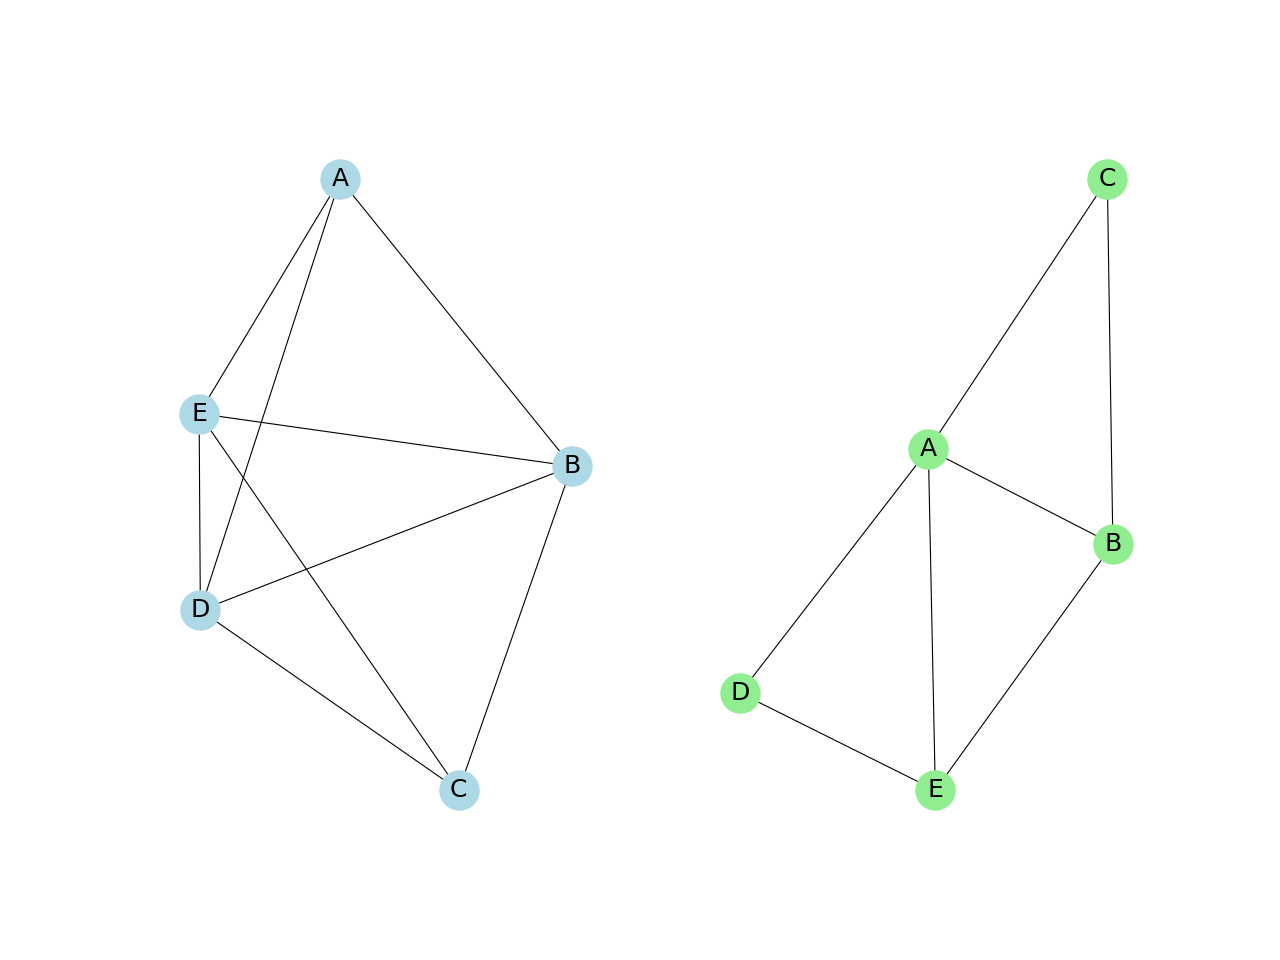
\includegraphics[width=1.0\textwidth]{Graphics/MatrixInNetwork.png}
    \caption{Links ist Netzwerk1 als Graph dargestellt und rechts Netzwerk2}\label{fig:MatrixInNetzwerk}
\end{figure}

Im Grunde können aber für jegliche Netzwerkanalysen beide Varianten verwendet werden. Jedoch werden in dieser Arbeit überwiegend Graphen zur Veranschaulichung und Matrizen für jegliche Berechnungen verwendet, da es leichter ist auf den Datentyp einer Matrix zuzugreifen. Das in Python bereits definierte und verwendete Paket heißt "NetworkX". Dies ist ein Python-Paket für die Erstellung, Bearbeitung und Untersuchung von Struktur, Dynamik und Funktionen komplexer Netzwerke. Dort ist es möglich, einige Features, welche ein Graph aufweist zu veranschaulichen \cite{NetworkX}. \\
In dieser Arbeit betrachten wir, wie in \ref{fig:MatrixInNetzwerk} unschwer zu erkenn ist, nur
ungewichtete Netzwerke, um die Zentralitätsmaße, beziehungsweise Netzwerkeigenschaften zu diskutieren.

\section{Einführung in die Grundstruktur von sozialen Netzwerken}
Ein soziales Netzwerk ist eine soziale Struktur, die zwischen Akteuren - Einzelpersonen oder Organisationen - besteht. Es zeigt die Art und Weise, wie Menschen und Organisationen durch verschiedene soziale Vertrautheiten verbunden sind, die von zufälligen Bekanntschaften bis hin zu engen familiären Bindungen reichen. Soziale Netzwerke bestehen aus Knotenpunkten und Verbindungen, deren Wechselwirkung nicht linear ist. Die Person oder Organisation, die am Netzwerk teilnimmt, wird als Knoten bezeichnet. Bindungen sind die verschiedenen Arten von Verbindungen zwischen diesen Knotenpunkten. Bindungen werden nach ihrer Stärke bewertet. Lockere Verbindungen, wie bloße Bekanntschaften, werden als schwache Verbindungen bezeichnet. Starke Verbindungen, wie z. B. Familien oder Cliquen, werden als starke Bindungen bezeichnet \cite{SNADefinition}. Beispiele für soziale Netzwerke sind unsere Gesellschaft, das Internet, unser Gehirn und zelluläre Interaktionen.
Doch welche grundsätzlichen Eigenschaften muss ein Netzwerk erfüllen, um als $"$soziales Netzwerk$"$ bezeichnet werden zu dürfen? 
Sozialwissenschaftler*innen haben drei Arten von Netzwerken untersucht: egozentrische, soziozentrische und systemoffene
Netzwerke. Egozentrische Netze sind Netze, die mit einem einzigen Knoten oder einer einzigen Person verbunden sind \cite{egocentric}. Um als Netze zu gelten, müssen diese Verbindungen nicht nur Listen von Personen oder Organisationen sein, sondern es müssen auch Informationen über die Verbindungen zwischen diesen Personen oder Organisationen enthalten sein. Im allgemeinen Sprachgebrauch, insbesondere wenn von sozialer Unterstützung die Rede ist, wird jede Liste als Netzwerk betrachtet. Eine Person, die eine große Anzahl guter Freunde hat, auf die sie auf die sie sich verlassen kann, wird ein großes "Netzwerk" genannt. Soziozentrische Netzwerke sind, wie Russell Bernard Bedeutung (persönliche Kommunikation), Netzwerke in einer Box. Netze mit offenen Systemen sind Netze, bei denen die Grenzen nicht unbedingt klar sind, sie liegen nicht in einer Box - zum Beispiel die Elite der Vereinigten Staaten oder die Verbindungen zwischen Unternehmen, oder die Kette der Beeinflusser einer bestimmten Entscheidung oder die Übernahme neuer Praktiken. In gewisser Weise sind dies die interessantesten Netzwerke. Sie sind auch am schwierigsten zu untersuchen \cite{charlesKadushin}. 

Diesen Teil werde ich zu einem anderen Zeitpunkt schreiben müssen weil ich keine Quellen finden, die es gut genug beschreiben was ich genau als Daten brauche.




%*****************************************
%*****************************************
%*****************************************
%*****************************************
%*****************************************